\documentclass[a4paper,11pt]{article}
\usepackage[style=mla,style=authoryear,backend=biber]{biblatex}
\renewcommand*{\nameyeardelim}{\addcomma\space}  % add comma between author and year
\usepackage{soul}
\usepackage{hyperref}
\usepackage[colorinlistoftodos]{todonotes}
\usepackage{calc}  % importent in order to import inkspace images
\usepackage[labelfont=bf]{caption}  % set caption label to bold
\usepackage{enumitem}  % to interrupt enumerations and resume
\usepackage{amsmath}
\usepackage{tabularx}  % alternative tabular package for the surveys
\newcolumntype{Y}{>{\centering\arraybackslash}X}  % for centered columns
\usepackage[toc,page]{appendix}

\addbibresource{bibliography.bib}

\graphicspath{ {images/}{graphics/} }

\newcommand{\definition}[1]{\emph{#1}}
\newcommand{\noriinline}[1]{\todo[author=Nori,inline,color=green]{#1}}
\newcommand{\nori}[1]{\todo[author=Nori,color=green]{#1}}
\newcommand{\myunderline}{\rule{2in}{.5pt}}

\title{Audio-Only Augmented Reality System for\\Social Interaction} 
\author{Tom Gurion}

\begin{document}
\maketitle

\listoftodos

\section{Introduction}

In the past 60 years the development of new technology has fundamentally transformed music creation and consumption (\cite{hargreaves99}).
One of the results of these transformations is interactive music systems (IMS), a concept that facilitating new ways of music creation and blurring the traditional distinction between instrument design, composition and performance (\cite{drummond09}).
In the recent years there are many attempts to provide IMS not only to the professional musicians but also directly accessible to the average user (\cite{stimulant13}).

This research follows this trend by exploring new possibilities for interactive music consumption.
In this work I will propose an audio-only augmented reality system for social interaction.

I designed and built an Android application that measures the relative position of the device from freely movable Bluetooth beacons.
Based on this information, an algorithm dynamically changes the music that the users hear in their earphones.

The interactive component of the system has already been assessed in a pilot experiment.
My preliminary results suggest that the system facilitated higher levels of user movement in space and enhanced social interactions, thereby displaying the potential of using audio-only augmented reality in future mobile applications.

Lastly, a more comprehensive experiment is suggested to revile more insights about the social interaction of using the proposed system in the context of a silent disco party.

\section{Literature review}

The current work is based on interdisciplinary research in several different domains.
The following sections will review those domains with emphasis on the projects, technologies and researches that serve as the groung for both my system development and its evaluation.

\subsection{The origins of IMS}

According to the Oxford Dictionary to ``interact'' is to ``act in such a way as to have an effect on each other''.
In the field of IMS actions and affects may be achieved using a broad spectrum of novel techniques, ranging from interactive sound installations to collaborations with robotic performers (\cite{drummond09}).

Traditionally, IMS merge development in several different threads such as music oriented programming languages as the MUSIC-N series and Max/MSP (\cite{mathews69}; \cite[p. 16]{winkler01}), standardization of technologies like MIDI (\cite{web:quinn}) and VST\footnote{Steinberg technologies: \href{http://www.steinberg.net/en/company/technologies.html}{www.steinberg.net/en/company/technologies.html}.} and the recent emergence of the ``makers culture'' (\cite{kuznetsov2010rise}), to facilitate new ways of music creation.

Since the beginning of the exploration in the field of IMS in the nineteen-sixties, different researchers and composers created systems that were designed to interact with performer in a live situation.
First example of this kind of interactive system was Gordon Mummas' Hornpipe, a specially designed electronic system that alters the audio input from the performer and creates an interactive loop between the player and the sound created by the electronics circuit (\cite[p. 12]{winkler01}).

Later, during the nineteen-seventies, musicians and researchers have started to use newly developed programming languages designed for musical applications, such as GROOVE or the MUSIC-N series (\cite{mathews70}; \cite{mathews69}).
As a pioneering technology for digital sound synthesis those programming languages gained wide acceptance in the music research community.

On another direction: in the nineteen-eighties a group of musical instruments manufacturers agreed on universal standard for sending and receiving musical information digitally, establishing the MIDI protocol (\cite{web:quinn}).
The standardization of sending and receiving information combined with the emergence of personal computers facilitated the creation of modern programing languages for musical applications.
Max/MSP, which began its development by Miller Puckette in 1986, may be a good example (\cite[p. 16]{winkler01}).
As opposed to early programming languages as GROOVE or the MUSIC-N series, most of those, personal computer based, languages still exist today and keep progressing\footnote{Max 6, the recent version of Max/MSP: \href{http://cycling74.com/products/max/}{cycling74.com/products/max/}.}.
Moreover, new music oriented programing languages continue to be developed, presenting features like ``on-the-fly'' programming\footnote{ChucK: \href{http://chuck.cs.princeton.edu/}{chuck.cs.princeton.edu/}.}, web capabilities\footnote{The Web audio API: \href{http://www.w3.org/TR/webaudio/}{www.w3.org/TR/webaudio/}.} or modular, multi-touch environment for live performance\footnote{Usine Hollyhock: \href{http://www.sensomusic.org/usine/}{www.sensomusic.org/usine/}.}.

Similar technological shifts also facilitated the usage of Digital Audio Workstations (DAW) as a common alternative to analog recording equipment in studios (\cite{leider:04}).
With the arrival of the VST as the common standard for signal processing plug-ins for DAW, computers became even more essential tool for music production.
This developments were concurrent to the emergence of live performance oriented DAW as Ableton Live\footnote{Ableton Live: \href{http://www.ableton.com/en/live/}{www.ableton.com/live/}.} and software based DJ setups at the late nineteen-nineties.

Another key event in the history of IMS is the appearance of the Arduino platform in 2006.
The Arduino is an easy to use hardware and software package intended for interactive objects or environments creation\footnote{Arduino: \href{http://arduino.cc/}{arduino.cc/}.}.
The platform opened the door for musicians to use more then just audio and MIDI to communicate with music creation software in interactive environment, mostly by translating physical properties into sound.

More generally, one could see the Arduino as an important part of the new ``makers'' movements, a technology-based extension of the ``do it yourself'' culture.
By creating what used to be purchased and by sharing this knowledge back with the community, the makers are a major driving force in the development of IMS nowadays (\cite{web:kirn12}).

\subsection{Interactive music systems for non-professional musicians}

Today, IMS meets the non-professional musician in various scenarios: interactive video clips, mobile and album applications, interactive sound installations and social DJing.
While these examples are typical they are only a small portion of novel ways where non professional can now participate in interactive music creation, interactive consumption of audiovisual content and musically enhanced social interactions.

% interactive video clips: Interlude, Chris Milk and Aaron Koblin
Interactive video clips expose some of the roles traditionally kept for the director to the viewers.
As a relatively new phenomena video clips like these become more and more prominent.
A notable example are the works by Chris Milk and Aaron Koblin, in which the video clip is run on a dedicated web page and response to the users by tracking their mouse, keyboard strokes or other inputs\footnote{Milk and Koblin's projects: \href{http://www.thewildernessdowntown.com/}{www.thewildernessdowntown.com/}; \href{http://www.ro.me/}{www.ro.me/}.}.
Similar approach can also be found in the interactive video clips by the startup Interlude\footnote{Interlude: \href{http://interlude.fm/}{interlude.fm/}.}, Becks' recent project ``Hello again''\footnote{Becks' ``Hello again'': \href{http://www.hello-again.com/beck360/}{www.hello-again.com/beck360/}.} and various additional sources.

% mobile applications: Smule and RjDj
A major factor that contributed to the development in the field of mobile applications for music creation is the continues increase in computational power of those devices.
For example, AutoRap turns speech into rap by slicing the syllables and map them according to different beat styles\footnote{Smules' AutoRap: \href{https://play.google.com/store/apps/details?id=com.smule.autorap}{https://play.google.com/store/apps/details?id=com.smule.autorap}.}.
Another examples are the applications by Brian Eno and Peter Chilvers which enable users to compose music using only visual element on the device screen\footnote{Generative music: \href{http://www.generativemusic.com/}{www.generativemusic.com/}.}.
Finally, RjDj uses the phones' sensors to create ambient sonification based on the users' interactions with the daily environment (\cite{web:rjdj})\label{rjdj}.

% album applications
Album applications is another new trend where artists releasing their music as interactive applications for mobile.
A notable example of this trend is the latest album of the Icelandic musician Bj\"{o}rk that accompanied each of the songs in the album with a separated interactive experience (\cite{stimulant13}).

% interactive sound installations: objects with sound, project ADA
Sound installations are specific type of installations located in the three dimensional space that communicate with their audience through sound.
In some interactive sound installations the main interaction is between the viewer and the installation itself (\cite{web:visnjic}; \cite{web:cardiff01}) where in others the main objective is to facilitate social interaction in which participants can interact with one another (\cite{eng03}; \cite{web:kirn12}; \cite{web:murray-browne13}).

% social DJing: DistributedDJ, the BLOB and playmysong
Recent projects suggest a framework of sharing the role of the DJ in a bar or party between the participants so they can choose the music by themselves and the playlist is generated dynamically by their musical taste (\cite{web:shaw}).
Most of those project are implemented as mobile applications and some of them even integrate social elements\footnote{Playmysong: \href{http://www.playmysong.com/}{www.playmysong.com/}; The BLOB \href{http://vimeo.com/7338120}{vimeo.com/7338120}.}.

\subsection{Technology dependent social networking}

Silent disco and flash mobs, the conceptual roots of this research, are examples of modern type of social behavior that rely on the fast growth of social media.
My proposal operates in the context of silent disco party and is inspired by flash mobs in the usage of new technologies to facilitate creative and artistic social interactions.

Silent disco is the phenomenon of partying where the music is heard through headphones instead of loudspeakers.
The new phenomena already changed the possibilities of an ordinary party, for example: having two DJs spin two completely different sets side by side at the same party where each participant has two channel wireless headphones, and can decide which DJ to listen to\footnote{Headphone Disco: \href{http://headphonedisco.com/show.php}{headphonedisco.com/show.php}.}.
Alternatively, having no DJ at all and letting each participant to choose what music to hear, individually, through his or her mobile device and headphones is also made possible by this setup.

Flash mobs is a public gathering of people organized through social media to perform a short act jointly.
The unique aspects of this relatively new phenomena have led researchers to suggest that flash mobs emergence is a significant event in the history of mobile communication (\cite{nicholson05}) and that it inherently reflects an artistic intent (\cite{brejzek10}).

\subsection{Social effects of music}

\noriinline{Tom, this section still lacks a coherent nerative, please integrate some of the McDermott, Josh paper and then try organize it a little better, overall the content is ok, but it doesn't add up to a story and sounds like data dump, a little more work here}

% Music as a way for communication.
% Music social function.
% The influence on individual self identity and interpersonal relationships as described by Hargreaves and North.
% Classification of personality dimensions, self-views and cognitive abilities according to musical preferences as suggested by Rentfrow and Gosling.
Music is known for being an important channel of social communication.
It provides musicians with the ability to share emotions and meanings without words and can produce deep feelings among listeners (\cite{hargreaves02}).
It is no surprise therefore, that the psychological functions of music in everyday life have been extensively studied.
Hargreaves and North extend those insights about music functionality to the social domain, explaining the social effects of music on the individual by means of self-identity, inter-personal relationships and mood (\cite*{hargreaves99}).
Other researches show high correlation between music preferences and wide array of personality dimensions (e.g.\ conscientiousness and openness) as well as self-views (e.g.\ political orientation) (\cite{rentfrow03}).
Some research have also pointing out to the importance of music styles in the definition of the individual identity (\cite{cook00}).

% introduction to music as an evolutionary adaptation
% use Huron 2001
Another point of view suggests that music might be an evolutionary adaptation.
A supportive evidence is the observation that human have neurological specialization for music processing.
In addition, archaeological evidences indicate that music making in human settlements exist for more that 40,000 years (\cite{Huron2001}).

% in group and between group functionality
% use Darwin Descent of Man, Brown 2000 and Hagen & Bryant 2003
If music is indeed an evolutionary adaptation, its survival value for the individual should be placed in question.
First attempt to answer this question could be found in Darwin's \textit{``Descent of Man''}, by the suggestion that music exist to support sexual selection.
Recent studies criticize this attitude by standing on some fundamental features of music, such as isometric rhythm and discrete pitches, that emphasize musics' synchronization characteristics at the group level, rather then in the individual level (\cite{Brown2000}).

According to Brown, music functionality could be described with regard to both within-group cooperation, promoting group identity and cohesion, as well as between-group competitiveness.
Furthermore, Hagen and Bryant suggest that music and dance originally evolved as a signaling system for the existence, as well as the quality, of a coalition between individuals, noting that humans are the only primate to create cooperative alliances between groups in the absence of consanguineal ties (\cite*{Hagen2003}).

% joint action
% use Kirschner & Tomasello 2010 and Knoblich et al. 2011
Indeed, recent studies show that join music making and dancing still increase group cohesion, pro-social commitment among the individuals of the group and the intent to share the same collective goals (\cite{Kirschner2010}; \cite{Knoblich2011}).

\subsection{Indoor positioning systems (IPS)}

The system I propose will require the ability to locate the positioning of the users within an indoor environment.
As we will shortly see, this is a non trivial requirement.

Today, the usage of outdoor positioning systems is unquestioned and achieved mainly by the General Positioning System (GPS) which is available in almost any modern phone.
On the other hand, IPS has not been standardized yet and therefor it is still not available to the average user (\cite{web:turetsky}).

Recent researches state that WiFi is a favored technology among IPS for mobile devices.
WiFi based systems can also enhance accuracy by applying inertial navigation using additional sensors of the device such as accelerometer, gyroscope, compass etc. (\cite{web:harrop}).
Note however that those solutions depend on the deployment of WiFi infrastructure in every indoor environment where positioning information in desired.

A relatively new technology in the world of indoor positioning systems, the Bluetooth low energy (LE)\footnote{Bluetooth LE: \href{http://www.bluetooth.com/Pages/low-energy-tech-info.aspx}{www.bluetooth.com/Pages/low-energy-tech-info.aspx}}, has already gained success with the adaption of the technology by Apple with their iBeacon IPS (\cite{web:danova}).
Estimote\footnote{Estimote: \href{http://estimote.com/}{estimote.com/}.}, one of the biggest iBeacon manufacturers, has recently reported that more then 10,000 developers are using their products (\cite{web:thompson}).

Apple are not the only company to adopt Bluetooth LE as an IPS. StickNFind are using the same technology similarly\footnote{StickNFind: \href{https://www.sticknfind.com}{www.sticknfind.com}.}; Android introduced built-in support for Bluetooth LE\footnote{Android Bluetooth LE: \href{http://developer.android.com/guide/topics/connectivity/bluetooth-le.html}{developer.android.com/guide/topics/connectivity/bluetooth-le.html}.} and there is even arduino shield (standard board extension) for it\footnote{Arduino shield: \href{http://redbearlab.com/bleshield/}{redbearlab.com/bleshield/}.}.

\subsection{Augmented reality}

According to Azuma ``AR enhances a users' perception of and interaction with the real world''.
This concept usually relates to the visual modality: ``AR systems integrate 3-D virtual objects into a 3-D real environment in real time'' (\cite{azuma97}).

Todays augmented reality systems include wearable devices that can superimposes a computer-generated image on a users' view of the real world (e.g\ Google glass\footnote{Google glass: \href{http://www.google.com/glass/start/}{www.google.com/glass/start/}.} and Meta\footnote{Meta: \href{https://www.spaceglasses.com/}{www.spaceglasses.com/}.}) and applications for mobile devices for several purposes ranging from driving aids (iOnRoad\footnote{iOnRoad: \href{http://www.ionroad.com/}{www.ionroad.com/}.}) to marketing (\cite{ikea}).

My work extend the definition of AR system from the visual to the auditory modality opening the door for more comprehensive experience of virtual environments.

\section{Research targets}

The system developed in this research is inspired by the concepts of IMS and intended for the average user. In this research I will focus on the two following targets:
\begin{enumerate}
	\item To propose and implement an audio-only augmented reality system for social interaction.
	Using the system, participants will be able to interact with one another as well as with systems' components and affect the structure of the music in a virtual space.
	\item To evaluate the social effects of the system usage in the context of a silent disco party mainly focusing thereby on the following research question: \emph{does the system elaborate social interaction between participants in an interactive silent disco party?}
\end{enumerate}

\section{System development}

\subsection{Rational}

In this section I will explain the rational for the choices of system implementation in the context of the above research targets.

\subsubsection{Mobile and Android}

Todays' mobile phone has transformed from being a communication tool into a key `social object' in everyday life, and as such it has a significant importance in shaping todays' society (\cite{srivastava05}).
The applications of this research are targeted for the general audience and therefor the entire research will be implemented for mobile.

The system will be developed for the Android operating system\footnote{Android OS: \href{http://www.android.com/}{www.android.com/}.}.
Choosing Android as the platform for my research has two main advantages:
\begin{enumerate}
	\item The Android system is a growing mobile system which dominates most of the market share today (\cite{web:idc}).
	\item By developing application for Android I have access to underlying Bluetooth properties such as received signal strength indicator (RSSI), which is essential for my implementation of the system as laid out in the next section.
\end{enumerate}

\subsubsection{Indoor positioning system}\label{methods:ips}

Although there are available techniques to implement IPS I have decided to develop a novel method from the following reasons:

\noriinline{Please add a sentence, that you decided to use beacons (elements that emit Bluetooth signal and therefore enable relative position) to measures positions, and than provide the reason for the choice. IF YOU DO NOT DEFINE BEACON THAN YOU HAVE TROUBLE TO EXPLAIN WHY RELATIVE POSITION IS A GOOD IDEA}

\begin{enumerate}
	\item Most of the techniques available nowadays require infrastructure.
	As a system influenced by flash mobs I wanted users to be able to use it anywhere without the effort involved in infrastructure deployment.
	\item Tracking the positioning of the participants is only required in the context of their relative position to some other mobile tokens in the system, therefore we do not need to track the absolute position of each participant in space (the world coordinate of their position).
	\item As opposed to system where high accuracy is required, the current research needs only limited accuracy.
	Being able to estimate if a participant is relatively close to another mobile token or far from it is generally satisfying.
	\item Although Bluetooth LE based solutions satisfy the above requirements only the most recent mobile devices support it.
\end{enumerate}

The system I have developed --- the Bluetooth Based Relative Indoor Positioning (BBRIP) system --- consists of some Bluetooth beacons, placed inside bundles of balloons, and an Android application.
It is build around distributed architecture and therefor runs separately, as an Android application, on each one of the participants phones.
The application repeatedly searches for nearby Bluetooth beacons.
Received signal strength indication (RSSI) is used as an estimation of the distance between the user and the beacon.

\subsubsection{libpd}\label{methods:libpd}

Advance audio processing is beyond the capabilities of the Android application programming interface and therefor, in order to apply sophisticate manipulations on the audio in real time, a more powerful audio engine was required.
In a personal computer environment the programming language Pure Data (Pd), originally written by Miller Puckette in the nineteen-nineties, is one of the leading open-source softwares for computer music\footnote{Pd: \href{http://puredata.info/}{puredata.info/}.}.
In this research I have decided to use ``libpd'', a thin layer on top of Pd that turns it into an embeddable audio library, as an audio engine (\cite[p. v]{brinkmann12}).

\subsubsection{System description}\label{systemdescription}

\begin{figure}[!htb]
	\centering
	\def\svgwidth{0.9\textwidth}
	\input{graphics/system_architecture.pdf_tex}
	\caption{System architecture}\label{fig:sys:architecture}
\end{figure}

Figure \ref{fig:sys:architecture} shows a schematic diagram of the system, which consist of an Android application and specially designed Bluetooth beacons ($BB1 - BB4$).
The BBRIP system is used to estimate the distance between the user and nearby Bluetooth beacon.
This estimation is then sent to a Pd patch through libpd, which plays an audio loop corresponding to the nearby beacon by one of the sound zone players $SZP1$ -- $SZP4$.
Every audio loop is identified by a distinct musical style which can be rhythmically and harmonically synchronized with other loops in almost endless combinations.

\begin{figure}[!htb]
	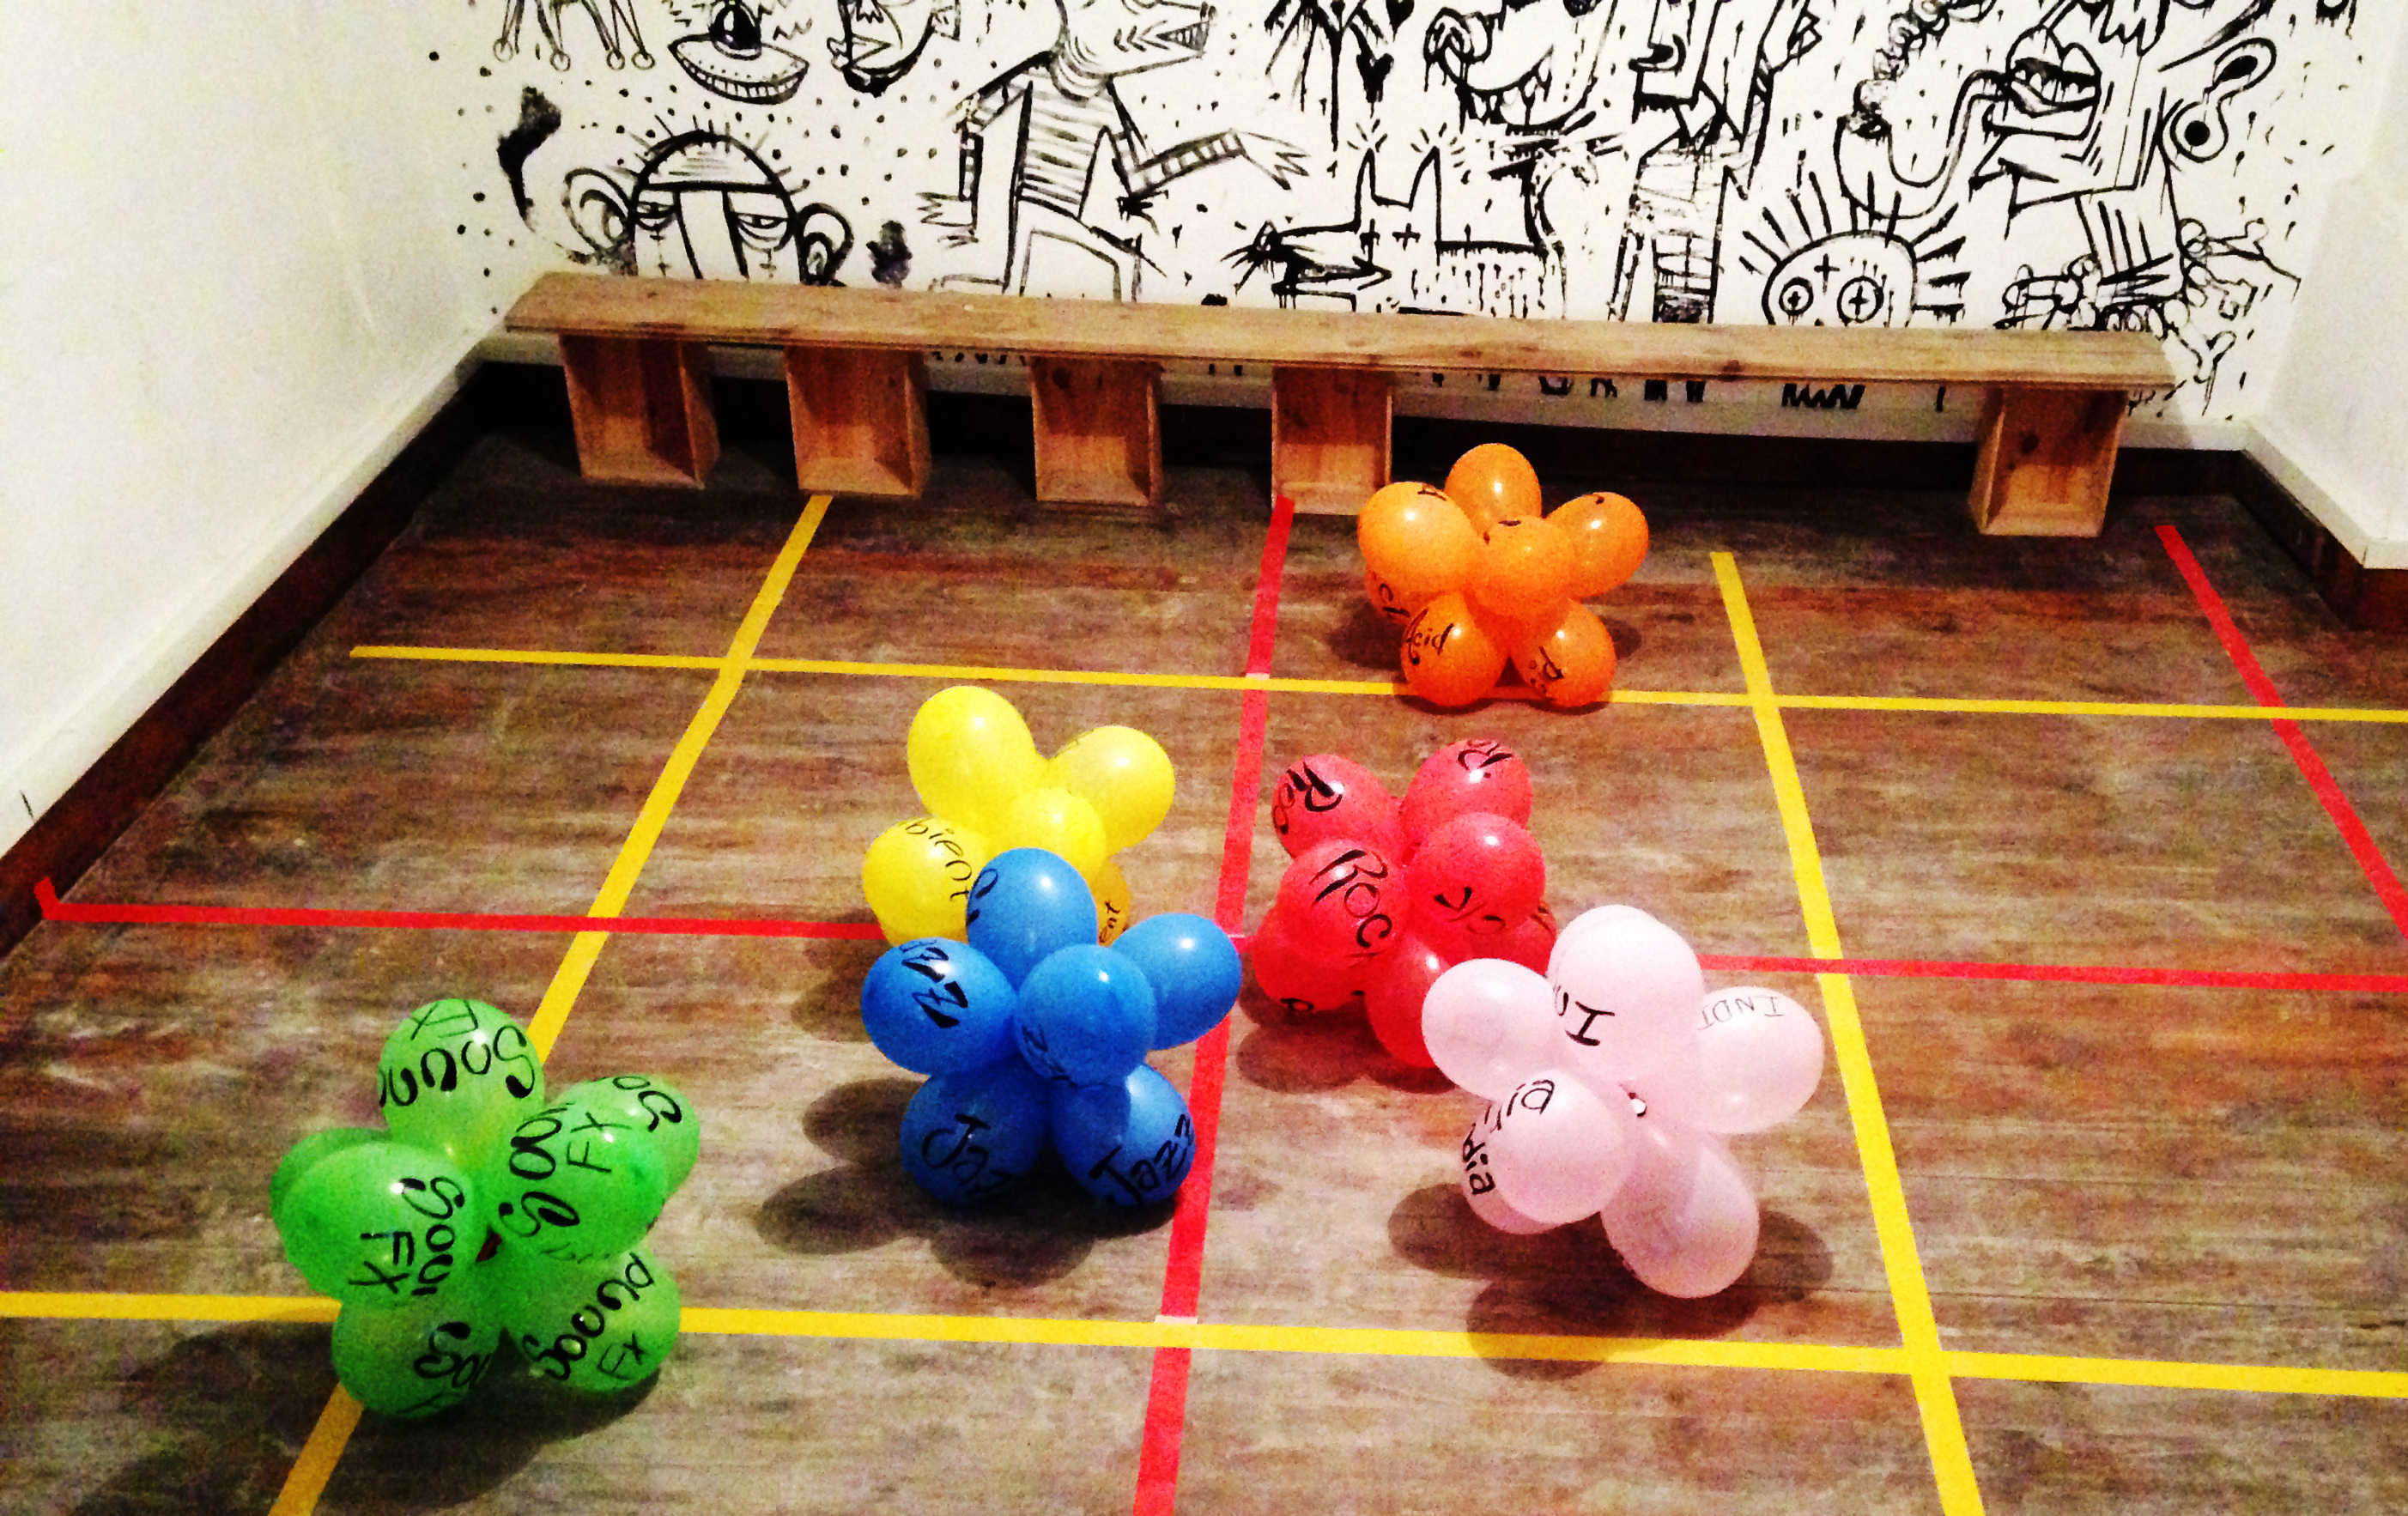
\includegraphics[width=\linewidth]{balloons}
	\caption{Balloon bundles on the dance floor}\label{fig:balloons}
\end{figure}

Figure \ref{fig:balloons} shows the systems' elements on the dance floor.
It consists of few balloon bundles, each one marked up with the name of a specific musical style (e.g.\ rock, jazz, Indian music).
A corresponding Bluetooth beacon is installed inside each one of those bundles.
After downloading and installing the Android application, strolling between the balloon bundles affects the music in ones headphones according to the relative distance from the bundles, creating a virtual ``sound zone'' around each one of them.
In addition, the distance from the center of each sound zones may affect the music in several different ways; for example by controlling volume, filter and granularity of the sound zone.
Lastly, participants can freely move the balloon bundles, thereby changing the structure of the music in the virtual space and making it socially interactive.

Figure \ref{fig:sys:participant_view} shows an overhead view of a possible scenario of participants using the system in a party.

\begin{figure}[!htb]
	\centering
	\def\svgwidth{0.9\textwidth}
	\input{graphics/system_participant_view.pdf_tex}
	\caption{The figure shows schematically two participants, $A$ and $B$, dancing around three Bluetooth beacons, corresponding to the rock, jazz and Indian music sound zones. Participant $A$ hear rock music and participant $B$ hear a mix between the jazz and the Indian music sound zones, which are rhythmically and harmonically synchronized with each other. A video demonstration of similar scenario can be found at \href{http://youtu.be/2kJoeD2iWBA}{youtu.be/2kJoeD2iWBA}.}\label{fig:sys:participant_view}
\end{figure}

\subsection{Implementation}

The implementation of the system could be described by two different processes: the development of the BBRIP system and the Android application that wraps it and is responsible for the audio processing.

\subsubsection{The BBRIP system}

The BBRIP system is my intent to develop an indoor positioning system that will satisfy the relatively simple requirements of the research as presented in chapter \ref{methods:ips}.

My implementation of the system is based on a specific element in the Bluetooth protocol -- the Received Signal Strength Indicator (RSSI) ({\cite{bray12}).
Each Bluetooth enabled device calculate RSSI values during Bluetooth discovery, when it finds a new device and before establishing connection.

\begin{figure}[!htb]
	\centering
	\def\svgwidth{\columnwidth}
  	\input{graphics/bbrip.pdf_tex}
	\caption{The BBRIP system}\label{fig:bbrip}
\end{figure}

As shown in figure \ref{fig:bbrip}, the BBRIP system continuously search for Bluetooth devices.
When a new device is found the RSSI value is extracted and send forward for processing.
From the first discovery in the Bluetooth discovery cycle the system keeps checking if the time since the last discovery exceeded a pre-defined timeout and if so it terminate the discovery.
This termination is important because naturally a device can only be discovered once in each Bluetooth discovery cycle and long period of time without new discoveries indicates that all of the nearby devices are already found.
Lastly, when the system sees that there is no Bluetooth discovery running (because of termination or simply the end of the discovery cycle), it starts a new one immediately.

Although the RSSI values extracted by the BBRIP system are not very precise as a distance estimation, I have found them sufficient enough in order to classify the distance between participants and beacons into useful ranges. In other words, RSSI values gives great indication if a participant is stands close to specific beacon (around 1 meter), in mediate range (2 to 3 meters) or in larger distance.

\subsubsection{ScenePlayer Plus}

The development of the Android application moved through different development stages.

First, I have developed an application that didn't use ``libpd'' at all (see chapter \ref{methods:libpd}).
In this early stage the only effect of getting close to, or far from a beacon was by changing the volume.
In addition, the limited sophistication of the built in audio library made fading in and out from the sound zones very non-flexible.

After finding the weakness of using the built in audio library of the Android application programming interface I have decided to implement the system using ``libpd''.
Although this implementation worked fine, it made a very tight coupling between the system development in the Android environment and the audio processing development in Pd.
Overall, this development phase was sufficient enough but in order to allow other musicians and developers to use the system I have started to look for more open architecture, that will maintain loosely coupled connection between the Android application and the Pd patch that drove the audio.

The last phase in the development of the system was to implement the BBRIP system into the open source Android application ``ScenePlayer''\footnote{ScenePlayer: \href{http://play.google.com/store/apps/details?id=org.puredata.android.scenes}{play.google.com/store/apps/details?id=org.puredata.android.scenes}.}, an Android port for the RjDj application mentioned in chapter \ref{rjdj}, and release it again as ``ScenePlayer Plus''\footnote{ScenePlayer Plus: \href{http://play.google.com/store/apps/details?id=com.nagasaki45.sceneplayerplus}{play.google.com/store/apps/details?id=com.nagasaki45.sceneplayerplus}.}.
The application exposes the Bluetooth RSSI values to the Pd patch as another sensor of the mobile device (e.g.\ accelerometer, compass and touchscreen).

\section{System evaluation}

In order to evaluate the social effects of the system usage I've decided to conduct controlled experiments.
For the sake of evaluating the system in its most natural designation, the context of the experiments has been chosen to be silent disco party.
The experiments main goal is to answer the research question: \emph{does the system elaborate social interaction between participants in an interactive silent disco party?}
In addition, an implied hypothesis is that participating in a party using the system strengthen the social relationships between participants even beyond the scope of the party.

Assessing the social interaction between participants is done using two main methods. By self reported information that the participants will fill in surveys before, during and after each experiment, and with objective measurements such as participants positioning tracking and their interaction with system components. 

The following sections present the pilot experiment that has been done, the motivation for a larger scope experiment and detailed explanation its of the design.

\subsection{Pilot experiment design}

\begin{figure}[!htb]
	\centering
	\def\svgwidth{0.95\columnwidth}
  	\input{graphics/pilot_design.pdf_tex}
	\caption{Pilot experiment design}\label{fig:pilot}
\end{figure}

Eighteen volunteers was invited to participate in an interactive silent disco party.
Each participant installed the Android application on his or her phone and filled pre/post party surveys that included questions regarding their musical background and preferences as well as system evaluation feedback.
The party consisted of four alternating interactive/control blocks of duration 5:40 minutes each (see figure \ref{fig:pilot}).
The participants were randomly assigned to two groups: $A$ and $B$, comprising the interactive and control blocks respectively\footnote{Group $A$ (interactive first) consists of 8 participants (4 females and 4 males) with mean age of 36.7 (s.d=12.3); group $B$ (control first) consists of 10 participants (3 females and 7 males) with mean age of 29.6 (s.d=10.2). Participants had a diverse musical background with 4.7 mean years of musical training (s.d=5.2).}.
They were generally informed that the experiment consists of interactive and control segments, however they were not informed about the exact schedule and timing of the blocks or the group assignments.
Both groups started the experiment together.
In the interactive blocks, the application generated music as described in chapter \ref{systemdescription}, whereas in the control blocks the participants heard recorded non-interactive music created in advance using the musical material of the interactive system\footnote{The control block music composed by Noam Elron (\href{http://www.noamelron.com}{www.noamelron.com}).}.

Interaction with the systems' components was assessed by counting the number of Bluetooth device discoveries made by each participants' phone during both the interactive and the control blocks.
In order to eliminate edge effects, we analyzed only the two middle blocks of the experiment.

\subsection{Preliminary results}

\begin{figure}[!htb]
\minipage{0.49\textwidth}
	\def\svgwidth{0.95\columnwidth}
  	\input{graphics/changing_location_in_space.pdf_tex}
	\caption{Changing location in space}\label{fig:location}
\endminipage\hfill
\minipage{0.49\textwidth}
	\def\svgwidth{0.95\columnwidth}
	\input{graphics/dancing_with_known_people.pdf_tex}
	\caption{Dancing with known people}\label{fig:known}
\endminipage\hfill
\end{figure}

In the post-party survey, participants self-reported significantly higher levels of movement (paired t-test, $t(15)=3.9$, $p<0.01$) using the system, compared with their behavior on other parties as reported in the pre-party survey.
Figure \ref{fig:location} shows that there was a significant difference (unpaired t-test, $t(33)=6.2$, $p<0.01$) in the mean response to these questions (at a scale of 1-3).

In order to objectively assess if participants moved more in space, we measured the counting of Bluetooth discoveries made by the applications' BBRIP system.
The results show slightly higher counts (paired t-test, $t(16)=1.7$, $p=0.06$, n.s) during the interactive blocks of the party compared with the control blocks. This suggests that the interactive components of the system facilitate greater participant movement in space, thereby offering more frequent opportunities for social interactions.
Indeed, in the post-party survey participants reported that they danced significantly less with people that they knew in advance, compared with their usual behavior (paired t-test, $t(14)=-2.5$, $p=0.01$).
Figure \ref{fig:known} shows that there was also a significant difference in the mean response to these questions in the pre/post surveys.
Overall, participants showed a slightly stronger tendency (paired t-test, $t(16)=1.46$ ,$p=0.08$, n.s) to participate in an interactive party in the post-party survey, compared with their answer to identical questions in the pre survey.

The preliminary results already demonstrate the potential for audio-only augmented reality to significantly enrich the experience of music consumption and its attendant social interaction.
We also show that this can be validated in a controlled experiment using both direct reports of subject and indirect objective measurements.

\subsection{Filling the gap}

Although the pilot experiment results already approve the hypothesis that the system usage enhance the social interaction between participants, it doesn't shed a light on the following points:

\begin{itemize}
	\item It does not distinct between participants that knew ones the other in advance.
	\item It does not show that the social effects of the system extends beyond the scope of the system usage.
\end{itemize}

The following experiment design tends to clear up those points.
First by assuming that participants in a party are pre-partitioned into groups of friends, and thereby a major effort will be made to gain better understanding of the behavior of those groups as a whole and the behavior of each participant as a member of a group.
Second, by using a control group that will not experience the interactive part of the system at all and will be compared, socially, to the experiment group before and after the experiment.

\subsection{Future experiment design}\label{methods:evaluation}

\subsubsection{Participants}

Thirty undergraduate and graduate-level students from the Music Department of Bar-Ilan university will participate in the experiment.
Their participation will rely on voluntarily will.

\subsubsection{Measurements}

The above research question will be fragmented into the following operational definitions and measurements\footnote{Complete version of each of the surveys below can be found in the appendix.}:
\begin{enumerate}
	\item \label{measure:partitioning} Participants will be asked to divide into groups of friends. The derived partitioning of the participants will be written for later use in the following measurements analysis.
	\item \label{measure:disperse} Using the above partitioning to groups of friends we can define the \definition{momentary center} of each group as the average positioning of its participants on the two dimensional plain of the dance floor.
	In addition, we can define the \definition{momentary disperse} of each group as

	\begin{equation*}
		\sum_{i=1}^n \frac{\sqrt{(x_i - \mu_x)^2 + (y_i - \mu_y)^2}}{n}
	\end{equation*}

	where $(x_i, y_i)$ are the positioning of the group members on the dance floor and $(\mu_x, \mu_y)$ is their \definition{momentary center}.
	Using the above definitions interaction between the members of one group with other participants will be evaluated by the disperse of the groups, when high disperse values indicate higher interactivity.
	\item \label{measure:groups} Using the above definitions, we can define \definition{momentary group disperse} as the disperse of the momentary centers themselves on the dance floor.
	With this regards low momentary group disperse values indicate higher interactivity.
	\item \label{measure:audio} The audio volume inside the experiment room will be used as an indication for the amount of `speaking' between participants and therefor as a measure of their engagement.
	\noriinline{but also could be saying that they do not really "into" the experiment because they talk instead of dance... can you elaborate or alternatively say that you do not commit to any of this interpretation but you want to use it as a measure of their social state and therefore predict that speaking "rate" would be}
	\item \label{measure:survey:social} Participants will fill social interaction survey.
	The survey will be used to asses interaction between participants by estimating social cohesiveness within in-group and out-group of each participant.
\end{enumerate}
In addition to measurements intended to assess the main research question.
The following operational definitions and measurements will be used in order to assess interaction with and satisfaction from the system.
\begin{enumerate}[resume]
	\item \label{measure:system} We will define \definition{momentary participant-system interaction} as the momentary distance of each participant from the closest Bluetooth beacon.
	Using the above definition high level of interaction of participant with the system will be indicated by low values of momentary participant-system interaction.
	\item \label{measure:survey:usability} Participants will fill system satisfaction survey, based on the System Usability Scale (\cite{brooke96}).
\end{enumerate}
Lastly, the following measurement will be used in order to eliminate possible differences between research groups and to allow future research based on the retrieved data.
\begin{enumerate}[resume]
	\item \label{measure:survey:musical} Participants will fill musical background survey, based on the Emmanuel College Music Background Questionnaire, basic version (\cite{web:zhao12}).
\end{enumerate}

\subsubsection{Apparatus}

In order to measure momentary disperse and group disperse as defined in measurements \ref{measure:disperse} and \ref{measure:groups} I will capture the experiment with video camera from above the dance floor.
Tracking the positioning of the participants will be done half manually by using software aids to record the manual tracking of participants, each at a time, using the computer mouse.
The results will be then processed using computational programming to conclude insights from the data.

Tracking data required in order to compute momentary participant-system interaction, as described in measurement \ref{measure:system}, will be derived the same way, by manually tracking each one of the system components in the video.

Audio volume (measurement \ref{measure:audio}) will be captured by a microphone and analyzed afterwards.

\subsubsection{Procedure}

Participants will be randomly allocated into two groups, group $A$ and group $B$\@.
Each group will participate in the experiment in different week, but in the same day of the week and same hour.

\begin{figure}[!htb]
	\centering
	\def\svgwidth{0.8\textwidth}
  	\input{graphics/procedure.pdf_tex}
	\caption{Experiment design}\label{fig:experiment}
\end{figure}

Participants will first fill a musical background survey as described in measurement \ref{measure:survey:musical}, followed by three \definition{experiment blocks}, followed by a system usability survey as described in measurement \ref{measure:survey:usability} (see figure \ref{fig:experiment}).
Each experiment block will consist of 15 minutes in which participants listen to music in their headphones, using their Android device and pre-installed application, and interact with other participants in the `silent disco' party.
Meanwhile, during each experiment block, measurements \ref{measure:disperse}, \ref{measure:groups}, \ref{measure:audio} and \ref{measure:system} will be collected.
Before each experiment block and after the last block each participant will fill the social interaction survey (measurement \ref{measure:survey:social}).

Each experiment block can be of one of the following types:
\begin{description}
	\item[Interactive:] In which the music generated by the Android application behaves as described in chapter \ref{systemdescription}.
	\item[Control:] In which the music generated by the Android application is pre-composed and based on the same musical materials as of the interactive system.
\end{description}

Participants of group $A$ will hear the experiment blocks: Control $\rightarrow$ Interactive $\rightarrow$ Control. Whereas participants of group $B$ will hear the experiment blocks: Control $\rightarrow$ Control $\rightarrow$ Control.

The procedure described above present several advantages in assessing the main research question:
First, the comparison between interactive and control blocks effects could be done as a between-group evaluation with relation to the second experiment block of each group.
Second, comparison between interactive and control blocks effects could also assessed as a withing-group evaluation between the first and the second, as well as the second and third blocks of group $A$, using group $B$ as a reference.
Lastly, effects on the social interaction beyond the scope of the interactive blocks will be assessed as a within-group evaluation between the first and the third blocks of group $A$, using group $B$ as a reference.

\begin{appendices}

\section[Musical background survey]{Musical background survey\\
	{\normalsize based on the Emmanuel College Music Background Questionnaire, basic version}}

Please first provide your basic information.

\begin{enumerate}
	\item Name: \myunderline
	\item Gender: Male / Female
	\item Age: \myunderline
	\item E-mail: \myunderline
\end{enumerate}
Please answer the following questions to the best of your knowledge.
\begin{enumerate}[resume]

	\item Please rate your overall interest in Music according to the following scale

	\begin{tabular}{c c c c c}
		Not interested & & Neutral & & Very interested \\
		1 & 2 & 3 & 4 & 5 \\
	\end{tabular}

	\item Please rate your overall Music ability according to the following scale

	\begin{tabular}{c c c c c}
		Poor & & Average & & Excellent \\
		1 & 2 & 3 & 4 & 5 \\
	\end{tabular}

	\item How many hours per week do you spend listening to music?

	\myunderline

	\item What genre(s) do you listen to most? (check all that apply)

	\begin{tabular}{l l}
		{[{ \ }]} & Classical \\
		{[{ \ }]} & Country \\
		{[{ \ }]} & Jazz \\
		{[{ \ }]} & Rock \\
		{[{ \ }]} & Pop \\
		{[{ \ }]} & Non-western \\
		{[{ \ }]} & Other: (please specify) \myunderline \\
	\end{tabular}

	\item Most of the time, when you listen to music, you are

	\begin{tabular}{l l}
		( \ ) & not focused on the music, attending to a different task \\
		( \ ) & passively listening \\
		( \ ) & highly aware of musical nuances such as key changes, harmonies, etc. \\
		( \ ) & actively engaged (sing along, tap the beat, etc.) \\
	\end{tabular}

	\item About how many hours of musical activity do you engage in each week currently? (e.g.\ practice, performance)

	\myunderline

	\item \label{appendix:music:ensamble}Have you ever participated in a musical ensemble?

	\begin{tabular}{l l}
		( \ ) No \\
		( \ ) Yes, instrumental ensemble \\
		( \ ) Yes, vocal ensemble \\
		( \ ) Yes, both instrumental and vocal \\
	\end{tabular}

	\item If you answered YES to question \ref{appendix:music:ensamble}, please indicate how many years you have participated in the music ensemble

	\myunderline \ years

	\item Please list any instrument(s) that you play (including voice) and the years you play each of them, beginning with your primary instrument:

	\begin{tabular}{c c}
		Instrument &  Years playing \\
		\myunderline & \myunderline \\
		\myunderline & \myunderline \\
		\myunderline & \myunderline \\
		\myunderline & \myunderline \\
	\end{tabular}
	
	\item \label{appendix:music:before_break}Have you ever had any formal training in music? (If you are a self-taught musician, please also answer YES)

	\begin{tabular}{l l}
		( \ ) & YES, I had a formal training in music \\
		( \ ) & YES, I consider myself a self-taught musician \\
		( \ ) & NO \\
	\end{tabular}

\end{enumerate}
Please continue this form if you answered YES to question \ref{appendix:music:before_break}, otherwise please go directly to question \ref{appendix:music:after_break}.
\begin{enumerate}[resume]

	\item What type(s) of music training have you had? (check all that apply)

	\begin{tabular}{l l}
		{[{ \ }]} & private/small group lessons in instrument and/or voice \\
		{[{ \ }]} & institutional training \\
		{[{ \ }]} & University degree in music - list degree: \\
		{[{ \ }]} & self-taught \\
		{[{ \ }]} & other (please specify): \myunderline \\
	\end{tabular}

 	\item At what age did you begin to study music?

 	\myunderline

 	\item How long did your formal music training last?

 	\myunderline \ years
 	\item How long has it been since you last participated in formal music lessons?

	\begin{tabular}{l l}
		( \ ) & Currently have one \\
		( \ ) & Or \myunderline \ years \\
	\end{tabular}

	\item \label{appendix:music:after_break}If there is anything else that you feel is interesting or important about your musical background, please comment below:

	\rule{4.5in}{.5pt} \\
	\rule{4.5in}{.5pt} \\
	\rule{4.5in}{.5pt} \\
	\rule{4.5in}{.5pt}.

\end{enumerate}

\section[System satisfaction survey]{System satisfaction survey\\
	{\normalsize based on the System Usability Scale}}

\begin{tabularx}{\textwidth}{p{2in} | Y Y Y Y Y }
	& Strongly disagree & & & & Strongly agree \\
	\hline
	I think that I would like to use this system frequently & 1 & 2 & 3 & 4 & 5 \\
	\hline
	I found the system unnecessarily complex & 1 & 2 & 3 & 4 & 5 \\
	\hline
	I thought the system was easy to use & 1 & 2 & 3 & 4 & 5 \\
	\hline
	I think that I would need the support of a technical person to be able to use this system & 1 & 2 & 3 & 4 & 5 \\
	\hline
	I found the various functions in this system were well integrated & 1 & 2 & 3 & 4 & 5 \\
	\hline
	I thought there was too much inconsistency in this system & 1 & 2 & 3 & 4 & 5 \\
	\hline
	I would imagine that most people would learn to use this system very quickly & 1 & 2 & 3 & 4 & 5 \\
	\hline
	I found the system very cumbersome to use & 1 & 2 & 3 & 4 & 5 \\
	\hline
	I felt very confident using the system & 1 & 2 & 3 & 4 & 5 \\
	\hline
	I needed to learn a lot of things before I could get going with this system & 1 & 2 & 3 & 4 & 5 \\
	\hline
\end{tabularx}

\end{appendices}

\sloppy  % fixing line breaks in bibliography
\printbibliography[title={Bibliography}]
\end{document}